\myChapter{Corporate Security Solutions for BYOD}\label{chap:byodSotA} 

\begin{flushright}{\slshape
   ... } \\ \medskip
    --- {}
\end{flushright}

\minitoc\mtcskip
\vfill

\lettrine{T}{he} way how users employ their devices has changed in the past few years; even the number of different devices per user is increasing because of the so-called Internet of Things \cite{weber2010internet}. Thanks to it, users have more flexibility since they can now use their devices to access company assets and continue working outside of the workplace. To allow this way of working, companies have started to adopt what has been called the Bring Your Own Device (BYOD) philosophy.

But data security and privacy are key factors for a company, and thus, in order to protect them, it is usual that the Chief Security Officer (CSO) of a company defines a set of Organizational Security Policies \cite{Opp_Security11}. Allowing a BYOD environment implies taking care of the risks that the use of personal devices can bring to
the company \cite{gangula2013survey}. For instance, the mixture between personal and professional information in these devices would allow the user to navigate inside social networks, where important data could be leaked in the event of a security incident.  

In this scenario several solutions that manage corporate security have appeared. Most of them are geared for both smartphones and desktop PCs, although some are implemented only for a certain platform. However, almost all of them try to be non-intrusive with regards to users' personal data, and also friendly and easy to use.

Even with the help of those solutions, it has been demonstrated that employees who aimlessly ignore company security policies are the main hazard for company security \cite{Adams_Users05}. In this sense, the tools that are appearing in the market aim to cope with the concept of seamless working experience on different devices. This concept is a methodology of work which allows users to start, or continue a working session, over multiple devices and locations, without any significant loss of data. This new situation might has a big impact from the point of view of the security \cite{Schu_SecPatterns05}, since company data borders have changed in the last years. Therefore, now the users can access important data from outside the enterprise, and possibly through a non completely secure channel.

As mentioned earlier, in the introduction, the aim of this thesis is to create a methodology that extracts knowledge and present it in the form of rules the CSO may include in the initial, fixed set of security policies. To this end, in this chapter we start by giving some concepts about enterprise security, following by some numbers about the usage of personal devices by the workforce during working time, and finally how are the companies coping with the BYOD philosophy. This can help us in detecting the features that are needed in these kind of tools but have not been yet implemented. Also, we introduce a BYOD system named MUSES, from Multi-platform Usable Endpoint Security, which has been developed within an European Project\footnote{\url{http://musesproject.eu/}} of the same name, and frames the contents of this thesis. MUSES is a dev\-ice\--in\-de\-pen\-dent end-to-end user-centric tool, based on a set of security rules defined as specifications of the Corporate Security Policies. Finally, in this chapter we propose a taxonomy to classify the features of BYOD systems. This taxonomy is used to present an overview of the found BYOD security solutions. Then, a comparison between the tools, including MUSES, is conducted, focusing on the advances beyond the state of the art that this novel system MUSES includes.

\section{Preliminary concepts and background about enterprise security}
\label{sec:preliminaryconcepts}

One of the tasks of a CSO is to elaborate an efficient set of Information Security Policies (ISPs), for controlling a certain, and already known, structure \cite{Opp_Security11}. This means that, until the appearance of BYOD, enterprises used to follow static security policies devoted to control an environment where the company assets and the devices were purchased and maintained by the company. Now that corporate networks are becoming dynamic for being adapted to this BYOD philosophy, there is an additional risk as employees' devices are not always company-owned. This means that the CSOs have to find the balance between having a fast response to any user action that might cause harm in terms of money loss, whilst trying not to intrude into users' privacy.

A needed security policy, or in this case, an ISP should deal with the way of protecting a certain organization's information against a security breach. Though there are standards, such as the ISO27002 or the Security Forum's Standard of Good Practice \cite{iso27002_isf}, and many guidelines \cite{SecPol09}, an ISP should be adapted depending on the characteristics of the community or organization that they are built for.

On the other hand, employee-owned devices like smartphones, can be both used for personal matters at work, and for continuing working outside of the workplace. Smartphones are more than simple mobile phones, and people who use them in their works have the possibility of maintaining a good balance between work and private life. For this reason, the risk of uncontrolled devices accessing to corporate assets in unsafe conditions, due to the number of new risks which are linked to smartphones \cite{gangula2013survey}, is increasing.

Usually, the enterprise network architecture is being adapted to cope with external attackers \cite{MIT05}. However, with the incorporation of BYOD, the threat is about corporate assets being compromised due to employees' devices with vulnerabilities \cite{android11}, or leaked because they are being accessed from a device connected through an insecure (public) network.

By knowing this, we should now consider more risky situations when designing a company's network architecture. Figure \ref{fig:proposed_diagram} shows our proposal, which can be used to start the study of solutions that may secure such a dynamic environment. It includes the possibility of having employee-owned mobile (smartphones and tablets) and portable (laptops) devices, and also the opportunity the employees have of connecting these devices either from inside or outside the company premises. Moreover, company's information assets are constantly accessed under these conditions, considering that an information asset means every \textit{piece of information} that has a \textit{value} (cost depending on the risk of being lost or leaked) for the company. It can be referred to files with sensitive information, as well as confidential mails, or even to company applications.

\begin{SCfigure}[tb]
\centering
	\includegraphics[scale =0.4] {gfx/byodSotA/proposed_diagram.eps}
	\caption{Architecture approach of an enterprise network, assuming that it has adopted the BYOD philosophy.}
	\label{fig:proposed_diagram}
\end{SCfigure}

The other issue to address is the elaboration of a good ISP, understandable for every user of the company, and more importantly, non-intrusive for him. A lot of researchers have studied the natural tendency of employees to comply with the ISP \cite{SecPolComp10,SecPolComp12,SecPolComp14}, reaching conclusions such as the employees compliance with the security policies increases by educating or training them in information security awareness \cite{SecPolComp09}, and decreases applying too much sanctions when a misuse or abuse occurs \cite{SecPolPenalty09}. Thus, in this chapter, for each reviewed tool, it is specified if the developers have taken into account the construction of ISPs, or even if they give some guidelines for building them. 

This situation leads to a need for protecting both the organization's and the users' parts, making non-interfering easy-to-follow ISPs, and leaving them to use their devices for personal purposes while working, without putting organization's information assets under risk. The compliance of these requirements would compose an End-to-End Security Solution (protecting both enterprise and employee), which is the motivation of the commented tools and is the aim of this thesis. All the details about this project are compiled in Appendix \ref{chap:appendixmuses}.

\section{Adoption of BYOD}
\label{sec:byodadoption}

Once the main concepts about why the companies need additional security have been discussed, we now need to understand the size of the problem, in terms of the diffusion of the BYOD philosophy. We need to establish, in terms of number of employees that use their personal devices at work and in which other places this philosophy is being adopted, how urgent is to provide solutions. This could help us to set the basis of the scenario we are going to deal with when building our methodology as a solution. After that, in the following chapter, we will review what solutions there exist and the possibilities they offer.

\subsection{BYOD in the enterprise}
\label{subsec:byodcompany}

The company Cisco made in 2012 a report called ``Connected World Technology Report'' \cite{cisco2012}. In this report they interviewed 1800 people from 18 different countries and ages from 18 to 30 about their personal and work life around their devices. The key results of this study are summarised as follows:

\begin{itemize}
	\item The 90\% of people said that they normally look at their smartphones as part of their waking up daily routine. This means that they like to be informed about any important matters before going to work and it is seen as positive by the IT professionals.
	\item When asked about they compulsively checking their notifications -- either text, emails, or social media updates -- , women admit to be more compulsive. Then, 85\% of women admit that they compulsively check their smartphones while 63\% of men say so.
	\item Social networks are a key too. 87\% of the respondants confirms they have a Facebook account and 10\% of those say to have it always connected. Less people reported to have a Twitter account, a 56\%, but 21\% of them said they tweeted at least once a day.
	\item Also, from their reported habits of use with regard of their smartphones -- if they use it while in bed, bathroom, having lunch with friends, and even driving -- the surveyers at Cisco estate that there are not marks between workday and personal time anymore.
	\item The majority of people (70\%) said that they use less than 10 smartphone applications -- apps -- regularly, whilst only 24\% confirmed to regularly use up to 25 apps.
	\item However, only a third of the surveyed people prefer smartphones than laptops, while slightly more than a third still prefer laptops over smartphones.
	\item With regard to the security policies of a company, a 40\% of the respondants say that their companies do not allow that company owned devices are used for non-work tasks. Nevertheless, not less than a 71\% of them admit that they often do not obey those policies and use the given devices for personal matters. It is curious than when asked to the IT professionals in the survey about this, around half of them think that their employees obey the policies.
	\item Finally, a 66\% of the people who responded in the survey agree with the statement ``employers should not track employees' online activities -- it's none of their business''.
\end{itemize}

Thomson \cite{thomson2012byod} also talks about this report, adding some detailed graphs in order to extract more conclusions. In his article, the author talks, on the one hand, about the users -- employees who demand BYOD -- and, on the other hand, about how the companies can adapt to them. Therefore, Thompson remarks that BYOD is important because only 39\% of the people suryeved by Cisco see themselves as responsible for securing their work devices and data. The rest think it is a matter for the IT department, the service provider, or both. With regard to the policies, a 12\% agreed with the IT policies being unfair or not being useful, and mostly half of the people surveyed asked for the company to understand their needs and to make flexible security policies. As suggestions, the author stands for intrusion prevention systems, reputation filtering, and user training in security.

The latest found report from Cisco is from 2014 \cite{cisco2014}. In this one they also interviewed people from 31 to 40 years old, in order to establish the differences between these two generations. However, the numbers are closely the same as in the report from 2012 \cite{cisco2012}.

On the other hand, a series of interviews and surveys were carried out during the MUSES project. They are detailed in \cite{musesD41, musesD42}.

The first document is devoted to identify what is called a ``Persona'', i.e. a user archetypes \cite{adlin2010essential}. To this end, both employees and CSOs were interviewed or presented a questionnaire about the devices they used and the security policies of their companies. Thus, the main conclusions from the study are summarised in what follows:

\begin{itemize}
	\item From the employees side, the study includes focus groups and an online questionnaire. In total, there were 21 people in the focus groups and 448 people responded to the online questionnaires, from different countries. All participants reported to be experienced with the use of technology.
	\begin{itemize}
		\item Half of the participants have company used devices, and when asked which ones, the most named were desktops, laptops, and smartphones in that order.
		\item It was observed that freelancers and self-employers were the ones who mostly tend to use their private devices for work purposes. Everyone agreed with their companies liking this practice because the employees are reachable beyond working time.
		\item When asked about security issues, the participantes relate this term to computer or software viruses. Actually, the way they consider they could lose their private data is by losing their smartphones; otherwise they do not think that somebody would be interested in stealing them.
		\item The majority of people surveyed assured they follow company security protocols such as having strong passwords and making periodic backups. But, as reported in the Cisco study \cite{cisco2012}, most of the people in the interviews agreed with the IT department being responsible for security.
		\item With respect to working remotely, more than a half (52'7\%) of the participants said to work up to 55\% of their working time remotely, although 50'7\% -- a little less -- said they work up to 55\% at their homes.
		\item Related to that, less than 20\% of the respondants reported that they do not work overtime. From the rest, the most part (39\%) spend between 2 and 8 hours working out of the working time, and only 11'3\% said to work more than 8 hours overtime. Nevertheless, the 72'4\% of these people assured that they are not getting paid for the extra work hours.
		\item In regard to the private devices for work purposes, in 20\% of the cases, the employer allows them. In spite of that, 44'6\% of employees responding say that they do not have an explicit security for that. Only 27'3\% declared that their company has a specific security policy for BYOD, and of those, 41'7\% say that they had it for at least 2 years.
		\item Overall, they agree with the statement ``personal and work issues are mixing more and more in my daily life''. Actually, the most proclaimed personal things the participants said they did with their corporate devices, and during work time, were checking private e-mails, making private calls, surfing the web, and checking social networks. At the same time, the top mentioned work related actions made out of the working time and with private devices were checking corporate e-mails, make work related phone calls, accessing files and data, and creating and editing documents, spreadsheets, and presentations.
		\item When asked about their security awareness, the 62\% of the people responding assured that they receive security policy information by their companies through e-mail, newsletter, or group discussions and workshops.
	\end{itemize}
	\item With regard to the CSOs, 15 were interviewed, from 3 different countries.
	\begin{itemize}
		\item 11 of the 15 participants have corporate smartphones and all used them also privately, even though only 9 of them had explicit persmission from their companies to do so.
		\item In addition, 10 out of 15 have a private smartphone, and 8 CSOs use it for work related matters, but only half of those were allowed by their companies.
		\item All 15 have company owned laptops. From the 10 that use them privately, only 6 have permission from the company.
		\item All the CSOs said that company laptops of computers have a firewall and antivirus software, and overall they agreed with their companies having strong security measures.
		\item Moreover, the participants said that in their companies, they apply one global security policy, although sometimes a different one is applied for external workers.
		\item In addition, they agreed with their companies not officially regulating BYOD even though it was permitted to some extent.
	\end{itemize}
\end{itemize}

In this scenario we can see that the employees demand the adoption of BYOD by these companies, and usually do not care about security policies, as they think that only the IT department is responsible for security. We can also conclude that the surveyed companies tend to allow BYOD practices without properly securing the environment. For these reasons, there is room for the development of a tool that helps companies in adopting BYOD, protecting important and valuable company assets at the time it makes the employees aware of the security and data loss.

\subsection{Other fields that have adopted BYOD}
\label{subsec:byodother}

The advantages BYOD brings make security policies gain traction in the education sector with an increasing number of schools around the world choosing to implement their own BYOD policies. In such environment, BYOD (also called Bring Your Own Technology or BYOT) refers to a technology model that allows students to bring their own devices to school for learning in the classroom \cite{sangani2013byod, song2014bring}. The adoption of BYOD in schools is supported by the fact that technology plays a leading role in
pupils/students' everyday lives and should, therefore, be an integral part of their learning. However, for most schools it is financially unsustainable to provide every student with the most appropriate up-to-date device. BYOD is therefore considered an attractive, cost-effective alternative, provided that many students usually own
devices that are superior and more up-to-date than those available in schools. BYOD at schools has several benefits as well such as personalising learning experiences, encouraging students' independent learning, and promoting anytime, anywhere learning opportunities.

\section{Research lines in BYOD}

Since BYOD policies started to appear in companies' day-to-day policies a lot of research has been done about the advantages and disadvantages of this approach \cite{singh2012byod}, as well as about how to properly implement it in order to respect privacy while trying to secure the resources \cite{scarfo2012new, ali2015analysis, de2015corporate}. These issues can be approached in different ways; Scarfo differentiates in \cite{scarfo2012new} two main ones: allowing the device to connect via desktop or application virtualisation, meaning enough control to avoid employee's devices monitorisation; or allowing the company to control devices via Mobile Device Management (MDM), which has to be legally agreed with the employee.

Ali et al. expand from Scarfo's study in \cite{ali2015analysis} reviewing both BYOD access control  and security models. The authors further distinguish between MDM and Kernel Modifications inside the security models, and conclude with the description of a proposed model which combines most of the reviewed solutions, i.e. MDM and Virtual Private Network (VPN) access together with an encrypted container for the accessed information depending on the level of restriction. However, from all the papers in \cite{ali2015analysis} claimed to enforce policies, only in \cite{rhee2013high} the authors actually describe how the policies are enforced by describing which data is monitored. In any case, none of the papers mention the application of Genetic Programming (GP) to the enforcement of the security policies, but other techniques such as the implementation of blacklists to avoid the installation of forbidden applications, or whitelists to allow only certain ones. These techniques can be useful with respect to the implementation of already defined security policies, but our method allows to discover new security policies, which in the case of black and white lists, can evolve them to include new and/or malicious applications.
There is an emerging research area in the field of BYOD. This is because, it is becoming a growing trend \cite{Garba15organisational}. There exist several methodological works on this subject. Samaras \cite{Samaras13SaaS} proposes a methodology design of a security architecture taking into account their logical design, logical architecture, security mechanisms and physical architecture. First, the business processes are studied and legal and security requirements are analyzed. After applying several controls the architecture is validated using different criteria: Correctness, Completeness, Usability and Flexibility. Romer \cite{Romer14BestPractices} proposes a set of best practices for BYOD security: centralize control and monitoring, protect confidential devices, increase trust with private clouds, connect to important services (such as Dropbox), block risky services and choose proven solutions.

Although some works present studies on the impact of BYOD in privacy \cite{Miller12Privacy} or relationship between workers productivity and stress \cite{Haejung12Door}, the most of them are focused in describing new systems and concepts in this paradigm. Scarfo presents in \cite{Scarfo12survey} a survey about the coming up methods in BYOD security. This survey summarises the research in two different approaches: {\em hands-off} versus {\em hand-on} devices. The first one proposes the use of some kind of virtualization or wrapping of the applications, while the latter is based in a tight control and monitoring of the device by the company.

An example of hands-off method is presented in the work by Gessner et al. \cite{Gessner13userfriendly}. This work mentions the importance of avoiding the modification of the underlying operating system (OS). Therefore, they propose the use of a ``container'' application, installed in the mobile device. This container is able to execute inside it the enterprise applications, acting as a barrier with the rest of the applications, and allowing direct communication with the enterprise VPN. The combination of this method, along cryptographic protocols and time-based sessions, offers a trade-off between security and usability. Also, this method avoids the modification of the underlying kernel of the device.

Other works propose the analysis of the applications before being installed. For example, in \cite{Armando14metamarket} a meta-market application is used to supervise the installation of new applications, using static analysis and code instrumentation techniques, taking into account the organizational security policies. A meta-market prototype is tested with Google Play market using a real world BYOD security policy \footnote{The US Government BYOD security guidelines.}.

It is interesting to mention that previous works are mainly focused in separating into hands-off vs hand-on devices, or static analysis techniques. However, neither of the papers found in bibliography establishes a taxonomy. In addition, the tools described in the reviewed works, do not implement any security policies adaptation methods, as the methodology we present in this thesis.

\section{Tools for corporate mobile security}
\label{sec:toolsreview}

Many tools for companies, as well as for devices, that help in adopting the BYOD philosophy have been released in the past years. From the point of view of the enterprise, there are some tools which offer the CSO ways to control the devices which enter into the system, for instance, and also to protect the employees' data by means of data encryption and data protection by requiring the use of strong and secure passwords. Other tools for managing a BYOD situation add to their features guidelines for the CSOs to develop good ISPs, like Good's BYOD solution (see Section \ref{subsec:othertools}). On the other hand, many solutions have been presented which are more focused on the device side, although they implement also the server side. This is the case, for instance, of Android for Work (see Section \ref{subsec:androidwork}). Some of those tools have influenced the development of the MUSES system  itself (Appendix \ref{chap:appendixmuses}), which can complement them, as adds other features that go beyond the state of the art. 

The products that have been reviewed were chosen either because they have appeared in top-10 web articles \cite{thor2013}, or they have been developed for the main smartphone platforms \cite{idc2014}. Actually, the selection process have been difficult, as some of the initially found tools or companies in the web were bought by others that we do review here. Also, because this market is still growing, there are not many solutions to review, and here we display the ones more alike to MUSES. This section introduces the most relevant features of these products, as they can be considered related to the MUSES objectives.

As these tools have several access levels, different detection methods, or diverse data control, there exist a number of aspects that the end-users need to take into account to validate if a product fits their needs. Therefore, we propose the next taxonomy in order to classify the BYOD tools described in this section.

\begin{itemize}
\item {\em Online or offline threat detection method}. This kind of tools can identify security threats during runtime (online) or before their implantation (offline). For example, using some kind of DM technique, such as classification methods, or merely the system administrator experience, can be used to generate rules before the deployment of the tool (offline) to detect threats in runtime. However, new rules cannot be added. On the contrary, a real-time adaptation using actual data sources, that modify the parameters of the detection system, follows an online scheme.
\item {\em Updatable or fixed information database}. This classification is related to the previous one. New information gathered by the system during runtime can be stored in a database to generate new rules. If this database is not changed during runtime, as in the offline example explained above, the database is {\em fixed}. An example could be the hand-coded rules of a firewall, such as {\em iptables}, obtained from an offline method. On the other hand, an updatable database, such as the system logs, that can be used to extract new information, may offer more valuable data source for dynamic adaptation mechanisms. However, it is not mandatory for an online threat detection method to use an updatable database, as current data may be analyzed and deleted once a new rule is created. 
\item {\em Based in an external service or standalone}: A standalone tool do not require a external service to be used. For example, a basic firewall. However, as mentioned by \cite{Romer14BestPractices} in previous section, a service for threat monitoring, or a private cloud usage are good practices to apply in BYOD.
\item {\em Invasive or non-invasive data access}. A system can be considered {\em invasive} if a user must use a certain tool to perform their job. For example, opening a specific browser provided by the tool, instead of the original device browser, such as Chrome of Safari. An example of an invasive marketplace is the one proposed by \cite{Armando14metamarket} and discussed in previous section. Instead, a {\em non-invasive} data access is transparent to the user. An example is a log analyzer daemon that updates other program configurations or sends information to the company server.
\item {\em Superuser or non-superuser system control}. Using a tool in superuser mode would add more information and control than a non-superuser running mode, as it can access to elements of the device usually forbidden for regular applications, such as network, logs or other devices. However using superuser control may lead to a lack of user privacy, as explained in \cite{Gessner13userfriendly}.
\end{itemize}


%----------------------------------------------------------------------------

\subsection{IBM Mobile Security}
\label{subsec:ibm}

One of the first companies who supported the BYOD model was IBM \cite{IBM_tool}, as they recognized the increase of employees who brought their personal smartphones or tablets into the workplace \cite{ibm11}. IBM provides different solutions divided into ``technology solutions'', and ``services'', and almost all are are mainly focused on the management of the devices in the system. Then, it might seem clear that the first disadvantage is not including all features in one system, but to make the companies choosing between one or another, or invest even more resources instead.

Main services offered by IBM can be divided into three categories: Mobile Enterprise Services, Hosted Mobile Device Security Management, and Enterprise Wireless Networks. However, here we only discuss the former, because it is the only one related to BYOD. Mobile Enterprise Services is offered as an integrated solution for smartphones and tablets as well, but then it is divided in different sub-services that the company has to acquire separately. Some of them are related, to cloud computing. Among them, there is one which is interesting for the scope of BYOD, the so-called `hosted vulnerability management'. This sub-service seems to implement one of the most important advantages of the MUSES system, the self-adaptation. IBM performs deep scans over the security incidents data, either by computer forensics analysis, if the incident happened, or by normal data, if the device was enough secure. They claim in their website \cite{ibmVulnMgm} that their tool is able to recognize new vulnerabilities or threats with enough accuracy. 

The specific IBM products related to BYOD security are included in their {\em MobileFirst} \footnote{\url{http://www.ibm.com/mobilefirst}} suite. MobileFirst is a set of mobile applications and services, based in big data analytics and cloud computing. It includes several products, such as a framework for app development (MobileFirst Platform), a Platform as a Service (BlueMix) or a threat detection system (Trusteer Rapport). However, the most interesting one with respect to this work scope, is {\em MobileFirst Protect}. This product, formerly known as {\em MaaS360} \footnote{\url{http://www.maas360.com/}}, is an MDM (Mobile Device Management) software to secure, monitor, and manage mobile devices. It uses a web portal in order to centralize the security and control policies. This allows the deployment of applications or backups, among other possibilities. However, MobileFirst Protect seems a typical MDM tool, which just applies the existing set of security policies. No further risk and trust analysis is performed, neither is included a refinement of the rules derived from the policies.

The main difference with MUSES in this case, is that MUSES includes the threat recognition feature feature in the system, without the need of purchasing the service separately and configuring the different parts. Another difference is the fact that IBM software is not open source as MUSES system is. Then, to verify the success of this feature is highly difficult, as they do not present statistics in their website either. In addition, this product also offers the possibility to work offline, though an initial online authentication is needed \cite{mobFirstAuth}. 
 
%----------------------------------------------------------------------------

\subsection{Sophos Mobile Control}
\label{subsec:sophos}

Contrarily to IBM's solution services, Sophos offers a whole product for securing BYOD environments, which is called Mobile Control \cite{Sophos_tool}. It is oriented to IT administration for mobile devices, and it can be deployed in two ways: on-premises, which means that all data and services remain in the servers of the company, and as Software as a Service (SaaS), so that the services are provided through Lightweight Directory Access Control (LDAP). LDAP is an application protocol for accessing and maintaining distributed directory information services over an Internet Protocol (IP) network.

The tool manages all employees' smartphones and tablets from a single-based console. This console monitors the devices since the initial set up and registration, until they log off. Remainder features are similar to IBM's product, adding some new such as the incorporation of a service called Malware and Web protection, so that there is no need for having a previously installed antivirus in the devices. Also, version 4.0 adds a new version of what has been called `Sophos Antivirus Engine', with offline detection capabilities.

With regard to compliance enforcement, the main goal of this Mobile Control tool is to give more importance to company security, instead of giving more flexibility to the users. But it has been demonstrated by Herath and Rao in \cite{SecPolPenalty09} that this practise can result in bad users' behavior, even if it was not on purpose. Thus, the company BYOD initiative should include an acceptable use policy to ensure that the users are aware of the measures that the company would take if a device breaches any ISPs. Sophos aims to reach this by doing three main tasks: First, by allowing setting up user and group-based security policies separately. Secondly, by a risk mitigation in which the actions to perform can be set according to the severity of the breach. For minor cases, the company might want to simply inform to the user, but if sensitive data is at risk, a remote wipe might be the chosen option. Finally, compliance check, by constantly performing scans to detect malware and putting the devices in quarantine when they are found infected.

Thus, given the fact that this tool is more focused on the company than in the user, it is worth to compare it to the MUSES system, as the latter tries to focus on the users, being user-centric. This means that is preferred to let the user know about a risky situation, rather than making them feel ``watched''. 

%----------------------------------------------------------------------------

\subsection{Samsung KNOX and Blackberry Balance}
\label{subsec:samsungblackberry}

Even though these two tools are provided by two different manufacturers, Samsung and Blackberry, they both have in common their situation, as they found problems in the market in spite of their features. On the one hand, Blackberry sales have been decreasing since 2010 \cite{Blackberry_sales}.
On the other hand, Samsung revealed at the Barcelona Mobile World Congress 2013 the KNOX application \cite{Samsung_mwc13}, which was expected to be available for its last Galaxy smartphone generation. Then, it was delayed and again presented in the same congress in 2014 \cite{Samsung_mwc14}, but still remained delayed until it was apparently found insecure \cite{Samsung_insecure}. Finally, Samsung decided to collaborate with Google in Android Work \cite{Samsung_android}, as mentioned in Section \ref{subsec:androidwork}.

With regard to their features, Samsung KNOX, as well as Blackberry Balance, are more focused on the device side, while the solutions mentioned in previous subsections were more centered in being tools for CSOs. This also means that they are not device-independent, as KNOX is only for Samsung devices and Balance is integrated in BlackBerry 10 \cite{Blackberry_tool}. Looking at their situation and problems, it could be thought that making a BYOD solution platform-dependent is counteractive, which is why MUSES is independent of the device platform.

The main feature of KNOX is the use of different containers, or environments, for business and personal sides. Each one includes its own graphical configuration, such as wallpapers, or colour themes, in order to be more easily recognized and distinguished by the user.
A password is required in order to enter into the business side and, once \textit{logged in} to this container, no more passwords are needed for the business applications. The applications approved by the company IT department must meet Samsung security standards and, though it has been said that KNOX is a device-focused solution, the company offered an API. This API would allow the company to access to over almost 205 predefined IT policies. With regard to information protection methods, data files saved by applications of each environment are encrypted with AES 256-bit algorithm, in such manner that only the appropriate container can access these files. In the same way, the user is not allowed to share data between the two environments. Figure \ref{fig:img_knox_01} shows the device architecture with three main parts, each one in charge of deploying some of the mentioned characteristics.

\begin{SCfigure}[tb]
	\centering
	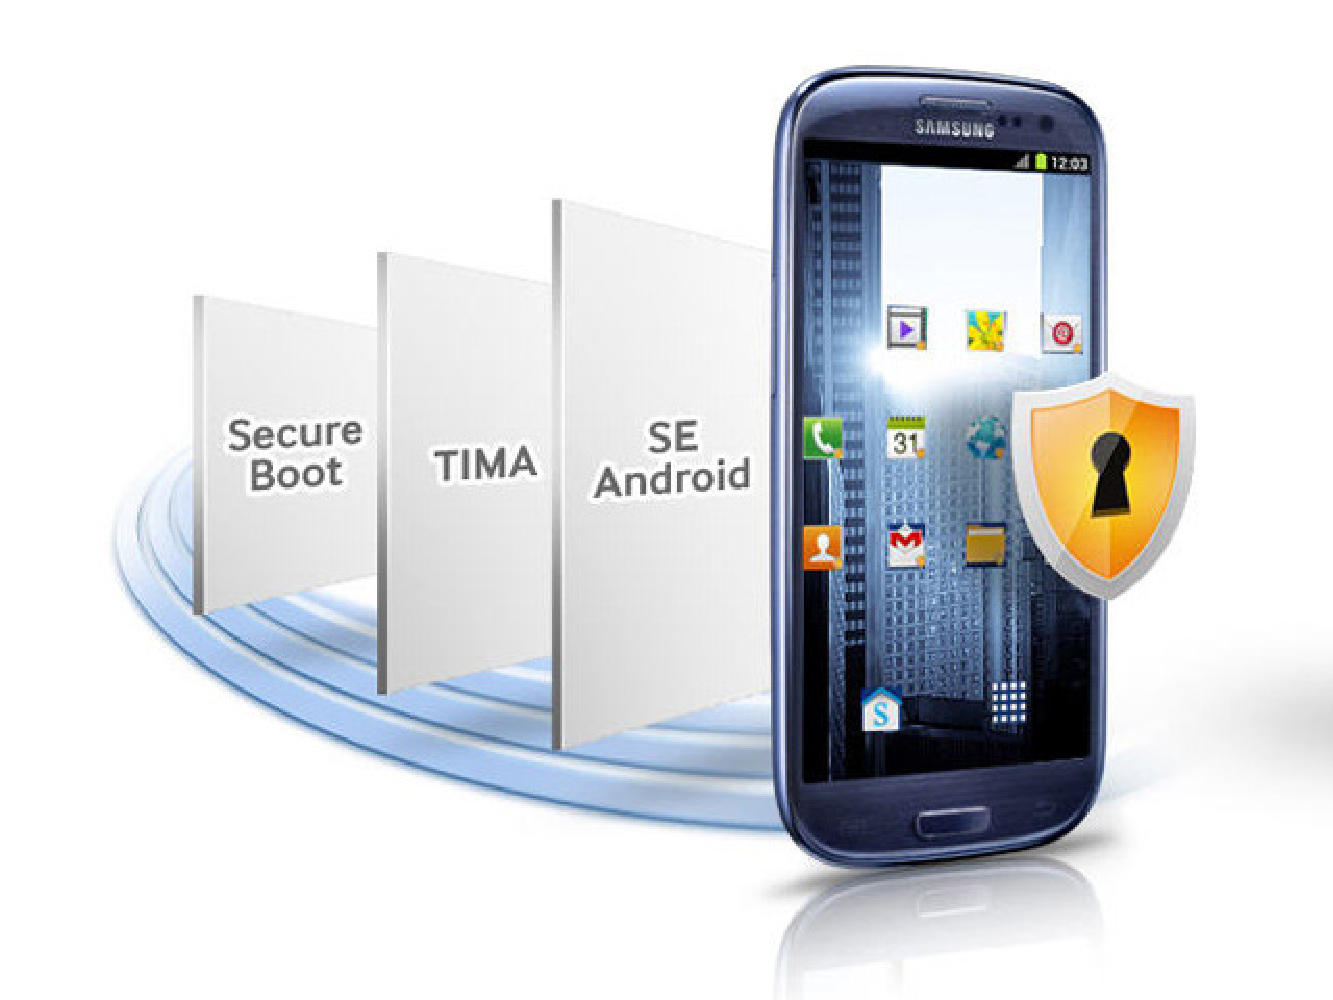
\includegraphics[scale =0.4] {gfx/byodSotA/samsung_knox.pdf}
	\caption{Samsung's Knox utility architecture. Source: \url{http://www.samsung.com/global/business/mobile/solution/security/samsung-knox}}
	\label{fig:img_knox_01}
\end{SCfigure}

Features in Blackberry Balance are similar. This security package was announced as a feature of BlackBerry 10. Nevertheless, it is available with BlackBerry Enterprise Service 10, which is a device management, security and app management for BlackBerry, iOS and Android devices. It is necessary to activate BlackBerry Balance for having available some security features, all related or similar to the aforementioned. For instance, as shown in Figure \ref{fig:blackberry_bal}, a message is displayed when the user tries to copy work data and then paste it into personal apps. Also, a user attempting for actions that are not permitted in the company ISP, or may cause secure work information to be in contact with personal applications, these actions will not be permitted. 

\begin{SCfigure}[tb]
	\centering
	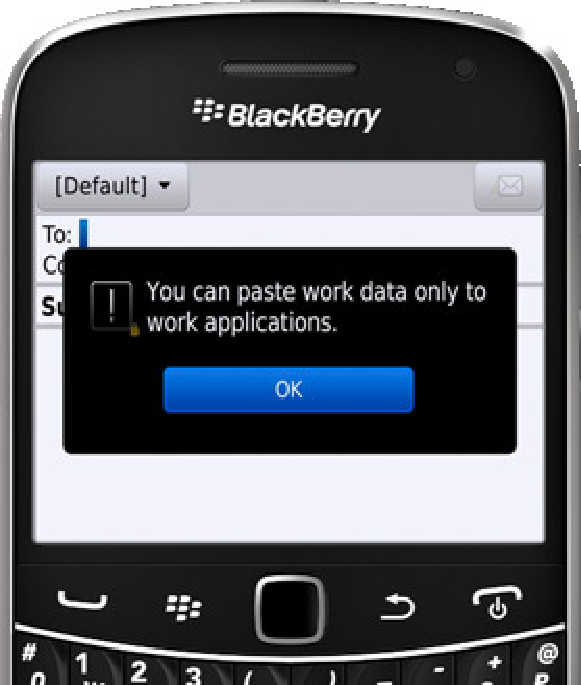
\includegraphics[scale =0.5] {gfx/byodSotA/Blackberry_balance.pdf}
	\caption{Displayed message in new Blackberry 10 when attepmting to copy sensitive company data. Source: \url{http://uk.blackberry.com/business/software/blackberry-balance.html}}
	\label{fig:blackberry_bal}
\end{SCfigure}

On the other side, while KNOX allows to \textit{push} policies from the server to the devices, so they are available offline, Blackberry Balance only allows to read documents in this mode. Finally, another known feature is also offered by Blackberry, so if the device gets lost, it is stolen, or if the employee leaves the organization, there is an option to wipe just work information which can be done remotely.

As a summary, Blackberry Balance has little opportunity if Blackberry sales continue to decrease, as well as Samsung KNOX, which is still out of the market. With this situation, MUSES could be a good choice, because is device-independent, and is available as an open source tool for both devices and servers.

%----------------------------------------------------------------------------

\subsection{Blackphone}
\label{subsec:blackphone}

On the device side, one of the most powerful solutions found in the BYOD state of the art is, apparently, to directly use a phone which has been developed with data security in mind such as the BlackPhone \cite{Blackphone}. It has its own Android-based operating system, called \textit{PrivatOS} \cite{Blackphone}, which includes a privacy-focused application store, called \textit{Silent Store}, that takes care of the problem of applications which ask for certain permissions that can lead, for instance, to personal data leakage \cite{gangula2013survey}. In Figure \ref{fig:blackphone} there is a list of the main advantages and security and privacy enhancements that PrivatOS has with respect to a standard Android OS. BlackPhone also allows a remote wiping of the data if the device is lost or stolen. The main disadvantage of this solution is either the enterprise having to make an investment and buy these smartphones to the employees or to make employees buy them, so they cannot use the device they already have. Both options are against the BYOD philosophy. On the contrary, the MUSES system proposed in this work is designed as device-independent.
Furthermore, the lack of information about this system makes it difficult to determine its real qualities.

\begin{SCfigure}[tb]
	\centering
	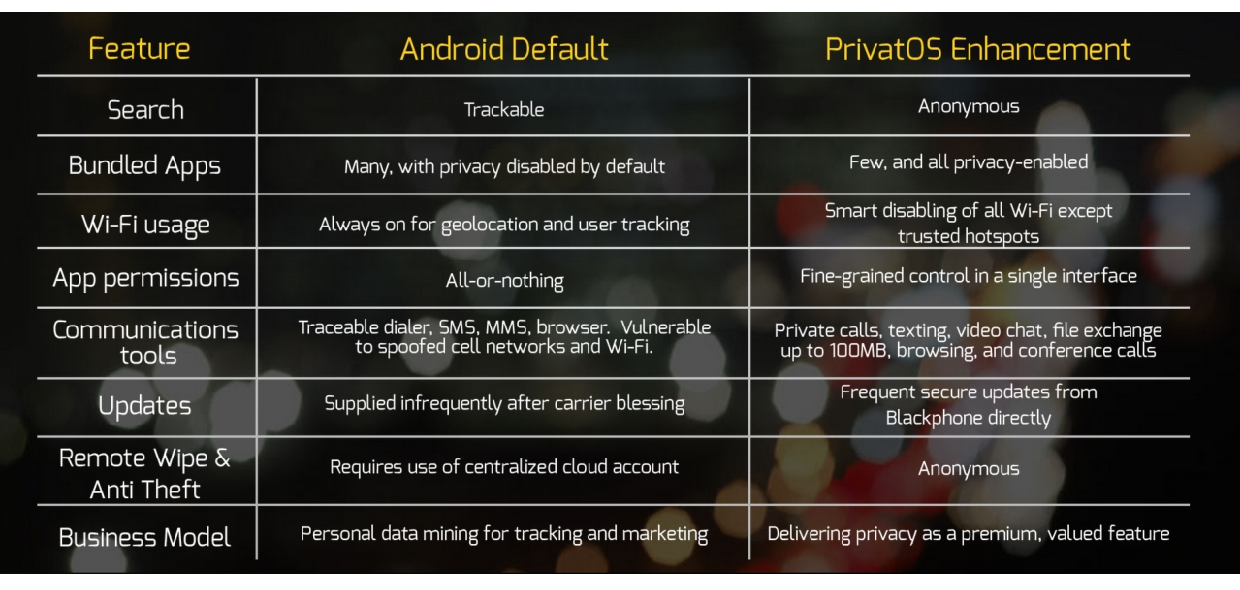
\includegraphics[scale =0.5] {gfx/byodSotA/blackphone.pdf}
	\caption{The features are compared with the ones in Android from the point of view os security and user privacy. Source: \url{https://www.blackphone.ch}}
	\label{fig:blackphone}
\end{SCfigure}

%----------------------------------------------------------------------------

\subsection{Android Work}
\label{subsec:androidwork}

This tool is the Google approach in the mobile enterprise security area, and  will run on Android 5.0 ``Lollipop''. It follows the idea of containers, previously presented in the Samsung KNOX description. Thus the container will be used to manage (encrypted) corporate data, and also to restrict what the users can do with them. This is called a ``dual-persona'' smartphone \cite{AndroidWork_review}.

This system is be strongly related to the Google Play market, as the applications will be `categorized'. Thus, Android Work provides the CSOs with a tool to define which apps would be allowed for being installed by the users and considered as corporate-related applications. Several enterprise-security aimed applications will be offered in the market, so the IT can decide which ones will be installed in the employees' devices. Also, they can manage the updates of these apps, in order to ensure that all the employees are up to date. For instance, one app could manage the creation of personal and work profiles, so the user just could access corporate assets after login in into the app. Moreover, the enterprise IT department could define specific security policies on these apps, in addition to the inherent protection that the container provides. However, the specifications of this tool \cite{AndroidWork_tool} do not include the ``self-adaptation'' as a feature, as the MUSES system does. 

Even though it does not analyze the system information for security rules evolution purposes, it offers policy management. Thus, the system will provide a framework for IT staff to manage business devices, but also, and more importantly, personal devices being used in a BYOD context. The CSO would give the employee an activation code in order to `connect' the smartphone to the enterprise and use this Android Work.
Therefore, IT admins will be able to specify which Google Play apps will be available for users to install through this work profile, including being able to provision apps to specific individuals or groups inside the company.

In addition to the work profiles, there will be considered other high-level ones with the ability to administrate the device from the corporate-security point of view, or as the owner, with all the privileges on the device.

Android Work presents only one advantage over MUSES, and roughly over all solutions, which is the ability to act over the Android kernel. The rest of tools only have permission for monitoring the running processes in the devices, while Android Work has, for instance, the ability to provide a `work' version of its native apps. MUSES, instead, depends on the developers to adapt their applications through a MUSES API, transforming them to MUSES Aware apps, as will be explained in Section \ref{subsec:client}. In any other case, and most of all with the ``self-adaptation'' feature of MUSES, it can be said that MUSES presents more advantages than the Google solution.

%----------------------------------------------------------------------------

\subsection{Multi-platform Usable Endpoint Security System}
\label{subsec:musestool}

MUSES is mainly a free, open-source, platform independent solution, and adopts the recommended best practices by Romer \cite{Romer14BestPractices}. These features make it a good alternative to most of the proprietary, close and system-specific tools presented in Section \ref{sec:toolsreview} (all but WSO2). In addition, most of the existing tools take into account only smartphones and tablets, but MUSES also covers laptops and company PCs, thus, it is not only for BYOD. Moreover, the companies which might want to work with one of the reviewed systems need a specific operating system in the server, being even more restrictive in some cases. This is specially remarkable in the case of the Blackphone, forcing the companies and the employees to purchase a specific device. MUSES is a good solution towards these cases, since it is a multi-platform system in both the client and the server.

This thesis is framed inside the European project MUSES (FP7-318508). The complete description of the MUSES project, along with the details of its architecture, can be found in Appendix \ref{chap:appendixmuses}.

%----------------------------------------------------------------------------

\subsection{Other tools}
\label{subsec:othertools}

There exist other corporate security-aimed tools inside the BYOD philosophy, of which there are less references on the Internet, but still we consider important for having similar features as MUSES. These tools are:

\subsubsection{WSO2 - Enterprise Mobility Manager}

WSO2 Enterprise Mobility Manager (WSO2 EMM) \cite{WSO2_tool} is an open source platform that also works with the BYOD program. Some of this WSO2 EMM key features are:

\begin{itemize}
  \item \textit{Mobile Device Management}: It is used to manage both user and corporate owned devices, providing support for Android and iOS at the moment. It should be noted that this tool allows tracking every enrolled device, as well as obtaining reports and analytics of their use.
  \item \textit{Mobile Application Management}: With regard to the software, this platform is able to allow or deny the use of applications on enrolled devices based on the role of the user or policies, thus restricting the use of some apps to certain users.
  \item \textit{Enterprise App Store}: This store provides users with both enterprise and public applications approved by the company.
  \item \textit{Mobile Data Security}: WSO2 also allows the user's data to be encrypted via password.
\end{itemize}

Although this tool also includes features such as device location, remote wipe, or encrypt storage, its main disadvantage is that it does not work in offline mode. In the documentation \cite{wso2Pol}, it is clearly stated that the policy compliance can be monitored while the devices are connected to the WSO2 EMM server. In addition, this tool seems to be only an MDM, without any refinement of the security policies.

\subsubsection{Good's Bring Your Own Device solution}

The philosophy followed by Good \cite{Good_tool} is similar to Samsung KNOX one: to create a secure container that places an unreachable partition between personal and business data in order to protect company assets. The solutions that they offer \cite{Good_tool} are similar than in the already described solutions. Their solution has been developed for the main OSs: iOS, Android, Windows phone, and also desktop computers with Windows. A Good's secure Network Operations Center (NOC) is introduced for dealing with the unauthorized devices, or for providing access to secure collaboration solutions (email, documents, calendar), the intranet, and both in-house or third-party mobile applications. Finally, Good offers best practice recommendations to help the company developing BYOD policies. A document can be accessed from Good's webpage \cite{Good_tool}, which contains several questions about ISPs and how to cope with all of them.

\subsubsection{Azzurri - Icon Mobilise}

It is a cloud-based service \cite{Azzurri_tool} to manage enterprise devices from the BYOD point of view, protecting sensitive corporate data and also letting the users enjoy them privately, by outsourcing the management of those devices to Azzurri.
 
\begin{itemize}
\item It offers a central deployment, administration and security control of all mobile devices regardless of their OS.
\item It manages and enforces security policies `over the air' for both corporate and employee-owned mobile devices.
\item It does it by enforcing passwords and providing mechanisms for remote lock.
\item It offers the ability to wipe, even selectively, corporate data email and contacts on the device if lost or stolen.
\end{itemize}


\subsubsection{Citrix - XenMobile}

XenMobile with the development environment called Worx App SDK, made by Citrix Systems, provides BYOD security services to companies using fine-grained policies to prevent users from performing unallowed actions \cite{WorxSDK}. For example using the mobile phone camera, GPS, or microphone. These policies can be turned on or off using its own GUI. Citrix is framework-enabled, and it is aware of the apps installed on the device. All the apps that are Worx-enabled are capable of interacting, and thus offering the user a better experience. This concept is similar to the `MUSES Aware' one, which was mentioned earlier in this section, and consists of adapting the applications to allow communications with the BYOD tools.

It is also important to point out that Citrix differentiates between apps used by the user privately and those used for business, locating both on a secure mobile container that is encrypted, and can be locked remotely for safety reasons. Another feature of Citrix is that it uses dedicated micro VPN to connect to Citrix-protected backend services.

Once the main tools and systems in this area have been introduced, in the following section our own system is presented, giving an overview on its general architecture. Moreover, we devote a subsection to describe its main features: the use of DM + ML techniques, and also its self-adaptation ability using CI methods, which compose the real difference with all the reviewed tools. 

\section{A comparison between tools}
\label{sec:comparison}

Table \ref{tab:taxonomy} summarizes the features of the main analyzed tools, with respect to the proposed taxonomy in Section \ref{sec:toolsreview}. Also, Table \ref{tab:features} shows the features of the analyzed products considering licenses, type of supported devices, and price.


\begin{SCtable}[][tb]
\resizebox{11cm}{!}{
\begin{tabular}{llllll}
\hline
\rowcolor{colorCorporativoSuave}{} & {\em \begin{tabular}[c]{@{}l@{}}Offline threat\\ detection method\end{tabular}} & {\em \begin{tabular}[c]{@{}l@{}}Updatable\\ database\end{tabular}} & {\em Standalone} & {\em \begin{tabular}[c]{@{}l@{}}Non-invasive\\ data access\end{tabular}} & {\em \begin{tabular}[c]{@{}l@{}}Superuser\\ system control\end{tabular}} \\\hline\hline
\rowcolor{colorCorporativoMasSuave}MUSES & \checkmark & \checkmark & \checkmark & \checkmark & \checkmark \\\hline
\rowcolor{colorCorporativoSuave}IBM Mobile Security &  &  & \checkmark &  &  \\ \hline
\rowcolor{colorCorporativoMasSuave}Sophos Mobile Control & \checkmark &  & \checkmark &  &  \\ \hline
\rowcolor{colorCorporativoSuave}Samsung KNOX & \checkmark &  & \checkmark & \checkmark & \checkmark \\ \hline
\rowcolor{colorCorporativoMasSuave}Blackberry Balance &  &  & \checkmark & \checkmark & \checkmark \\ \hline
\rowcolor{colorCorporativoSuave}Blackphone & - & - & \checkmark & \checkmark & \checkmark \\ \hline
\rowcolor{colorCorporativoMasSuave}Android for Work & \checkmark &  & \checkmark & \checkmark & \checkmark \\ \hline\hline
\end{tabular}
}
\caption{Features of the analysed tools with regard to the proposed taxonomy to classify BYOD systems.}
\label{tab:taxonomy}
\end{SCtable}

\begin{SCtable}[][tb]
\resizebox{11cm}{!}{
\begin{tabular}{llll}
\hline
\rowcolor{colorCorporativoSuave}{} & {\em License} & {\em Devices} & {\em Price} \\\hline\hline
\rowcolor{colorCorporativoMasSuave}MUSES & OpenSource & \begin{tabular}[c]{@{}l@{}}Android, iOS,\\Windows 8.1,\\Windows Phone\end{tabular} & Free \\\hline
\rowcolor{colorCorporativoSuave}IBM Mobile Security& Proprietary & \begin{tabular}[c]{@{}l@{}}Android, iOS,\\Windows Phone,\\Blackberry\end{tabular} & By request \\ \hline
\rowcolor{colorCorporativoMasSuave}Sophos Mobile Control & Proprietary & \begin{tabular}[c]{@{}l@{}}Android, iOS,\\Windows Phone\end{tabular} & By request \\ \hline
\rowcolor{colorCorporativoSuave}Samsung KNOX & Proprietary & \begin{tabular}[c]{@{}l@{}}Android, iOS,\\Samsung devices\end{tabular} & \begin{tabular}[c]{@{}l@{}}12\$ per\\year/device\end{tabular} \\ \hline
\rowcolor{colorCorporativoMasSuave}Blackphone & Proprietary & Own device & 120\$ per year \\ \hline
\rowcolor{colorCorporativoSuave}Android for Work & Proprietary & \begin{tabular}[c]{@{}l@{}}Android,\\devices with\\Chrome browser\end{tabular} & \begin{tabular}[c]{@{}l@{}}12\$ per\\month/user\end{tabular} \\ \hline\hline
\end{tabular}
}
\caption{Features of the analysed products considering licenses, type of devices and OS, and price..}
\label{tab:features}
\end{SCtable}


Another comparison would be that the existing products are mostly policy-based, while MUSES makes its decisions not only considering policies, but also based on the terminals and users context, such as connection properties, or trust value of the device, to really understand the real risk that comes with a specific action.

Also related to this issue, a very big advantage of the MUSES system that is not present in the other solutions is its self-adaptivity power. The proposed system uses different methods to create new security rules, being their aim to cover new vulnerabilities or threats. Thus, MUSES is able to adapt to changes by applying classification techniques to create new rules, and then refining the whole set of existing policies. Additionally, MUSES is able to discover new threats by a combination of real-time risk and trust analysis plus a classifier trained with all the occurred events in the system.

However, MUSES presents a limitation regarding the enhance of rules, since, in principle, it cannot predict or generate rules for dealing
with unexpected or unknown events, which could lead to a security incident. The philosophy is that the initial set of rules, defined by the CSO, should be very restrictive regarding possible unexpected users' behaviours or events, in order to avoid as much security incidents as possible. As the system works, MUSES would be able to define new rules through refinement which could get an associated decision after the corresponding events have happened. Thus, this will lead to obtaining an optimal set of security rules.

In addition, MUSES can also infer or create new rules using computational intelligence techniques. These rules could deal with unexpected situations not previously happened, but must be previously approved by the CSO. Of course, everything is constrained by the available set of sensors which, in turn, define the possible information that MUSES will analyze and use in the refinement and inference processes.

Moreover, another clear improvement over the rest is that MUSES can work in both online and offline modes, depending on the client being able to connect with the server or not, which favours the real-time decision making process.

These are not only advantages of MUSES over the existing products, but also a progress beyond the state of the art in some fields like risk and trust analysis, event correlation, and human-computer interaction (HCI).

First, as mentioned previously, it  implements a self-adaptive event correlation, including a novel hybrid technique of rule refinement and rule adjustment extracting relevant information from processing huge amounts of data. Then, the project defines a new approach to risk management taking into account threats, with their costs, as well as the innovative concept of opportunity: the following beneficial outcome from a situation on which, for instance, a user is able to work while waiting at the airport if the risk is low enough. 

As far as the HCI is concerned, in Section \ref{sec:preliminaryconcepts} we talked about how it has been demonstrated by Shaw et al. \cite{SecPolComp09} and Herath et al. \cite{SecPolPenalty09} that the compliance of the employees of a company, with respect to the security policies, increases by educating them and decreases by punishing them. Therefore, the fact that MUSES is focused in avoiding security incidents due to users' unawareness of the ISPs, it sets up a significant advance in the state of the art. This is because not only the incident is avoided, but the user is educated, which at the same time avoids future risky situations.
With regard to device monitoring, MUSES  also take into account the so-called context observation, by which private or professional scenarios can be detected, or predicted, based on advanced machine learning techniques. Finally, the project is concerned about legal compliance in regards of Information Security Policies, so that it  contributes to the proposal for the EU Data Protection: legal binding force and legal certainty of company policies, and end-user responsibility.

With regard to the scientific contribution of the system, one of the main differences with respect to previous works is the consideration of security threats `brought' by the user's behavior inside the system, i.e. through interaction or events, rather than more general and external threats. Moreover, the techniques to be used in MUSES  works with real data, as a difference to several research works which consider simulated data.

Authors have used DM techniques in previous works, but usually aiming for a specific general objective, for instance the detection of threats such as botnet \cite{botnet_detection_clustering_09}, or the recognition of anomalies \cite{feature_selection_anomalies_08}. However, these works do not contemplate any process to improve the system as the refinement phase in MUSES.

There are some proposals in which security policies are inferred or refined \cite{inferring_policies_socialnetworks_09,policy_generation_clustering_10}, but they do not affect the ISPs as in MUSES, and they are not based on the user's behaviour in order to do this.

GP has been previously proposed in bibliography \cite{rule_generation_gp_09,sec_policy_evolution_gp_08}, even for creating new policies or rules in a security-aimed sense. In any case they do not affect the ISPs and moreover, our proposed evaluation functions, completely integrated in the system, for the refinement and inference approaches are novel.

With respect to GA, they have been extensively used in this scope in the literature, mainly for the detection of anomalies and intrusions rather than for optimization, as it is used in the proposed system. However, there are some examples that could be used as model for our approach, such as \cite{EAs_securitycosts-kirta,risk_reduction_ga_12}.
